% Options for packages loaded elsewhere
\PassOptionsToPackage{unicode}{hyperref}
\PassOptionsToPackage{hyphens}{url}
\PassOptionsToPackage{dvipsnames,svgnames,x11names}{xcolor}
%
\documentclass[
  letterpaper,
  DIV=11,
  numbers=noendperiod]{scrreprt}

\usepackage{amsmath,amssymb}
\usepackage{iftex}
\ifPDFTeX
  \usepackage[T1]{fontenc}
  \usepackage[utf8]{inputenc}
  \usepackage{textcomp} % provide euro and other symbols
\else % if luatex or xetex
  \usepackage{unicode-math}
  \defaultfontfeatures{Scale=MatchLowercase}
  \defaultfontfeatures[\rmfamily]{Ligatures=TeX,Scale=1}
\fi
\usepackage{lmodern}
\ifPDFTeX\else  
    % xetex/luatex font selection
\fi
% Use upquote if available, for straight quotes in verbatim environments
\IfFileExists{upquote.sty}{\usepackage{upquote}}{}
\IfFileExists{microtype.sty}{% use microtype if available
  \usepackage[]{microtype}
  \UseMicrotypeSet[protrusion]{basicmath} % disable protrusion for tt fonts
}{}
\makeatletter
\@ifundefined{KOMAClassName}{% if non-KOMA class
  \IfFileExists{parskip.sty}{%
    \usepackage{parskip}
  }{% else
    \setlength{\parindent}{0pt}
    \setlength{\parskip}{6pt plus 2pt minus 1pt}}
}{% if KOMA class
  \KOMAoptions{parskip=half}}
\makeatother
\usepackage{xcolor}
\setlength{\emergencystretch}{3em} % prevent overfull lines
\setcounter{secnumdepth}{5}
% Make \paragraph and \subparagraph free-standing
\ifx\paragraph\undefined\else
  \let\oldparagraph\paragraph
  \renewcommand{\paragraph}[1]{\oldparagraph{#1}\mbox{}}
\fi
\ifx\subparagraph\undefined\else
  \let\oldsubparagraph\subparagraph
  \renewcommand{\subparagraph}[1]{\oldsubparagraph{#1}\mbox{}}
\fi


\providecommand{\tightlist}{%
  \setlength{\itemsep}{0pt}\setlength{\parskip}{0pt}}\usepackage{longtable,booktabs,array}
\usepackage{calc} % for calculating minipage widths
% Correct order of tables after \paragraph or \subparagraph
\usepackage{etoolbox}
\makeatletter
\patchcmd\longtable{\par}{\if@noskipsec\mbox{}\fi\par}{}{}
\makeatother
% Allow footnotes in longtable head/foot
\IfFileExists{footnotehyper.sty}{\usepackage{footnotehyper}}{\usepackage{footnote}}
\makesavenoteenv{longtable}
\usepackage{graphicx}
\makeatletter
\def\maxwidth{\ifdim\Gin@nat@width>\linewidth\linewidth\else\Gin@nat@width\fi}
\def\maxheight{\ifdim\Gin@nat@height>\textheight\textheight\else\Gin@nat@height\fi}
\makeatother
% Scale images if necessary, so that they will not overflow the page
% margins by default, and it is still possible to overwrite the defaults
% using explicit options in \includegraphics[width, height, ...]{}
\setkeys{Gin}{width=\maxwidth,height=\maxheight,keepaspectratio}
% Set default figure placement to htbp
\makeatletter
\def\fps@figure{htbp}
\makeatother
% definitions for citeproc citations
\NewDocumentCommand\citeproctext{}{}
\NewDocumentCommand\citeproc{mm}{%
  \begingroup\def\citeproctext{#2}\cite{#1}\endgroup}
\makeatletter
 % allow citations to break across lines
 \let\@cite@ofmt\@firstofone
 % avoid brackets around text for \cite:
 \def\@biblabel#1{}
 \def\@cite#1#2{{#1\if@tempswa , #2\fi}}
\makeatother
\newlength{\cslhangindent}
\setlength{\cslhangindent}{1.5em}
\newlength{\csllabelwidth}
\setlength{\csllabelwidth}{3em}
\newenvironment{CSLReferences}[2] % #1 hanging-indent, #2 entry-spacing
 {\begin{list}{}{%
  \setlength{\itemindent}{0pt}
  \setlength{\leftmargin}{0pt}
  \setlength{\parsep}{0pt}
  % turn on hanging indent if param 1 is 1
  \ifodd #1
   \setlength{\leftmargin}{\cslhangindent}
   \setlength{\itemindent}{-1\cslhangindent}
  \fi
  % set entry spacing
  \setlength{\itemsep}{#2\baselineskip}}}
 {\end{list}}
\usepackage{calc}
\newcommand{\CSLBlock}[1]{\hfill\break\parbox[t]{\linewidth}{\strut\ignorespaces#1\strut}}
\newcommand{\CSLLeftMargin}[1]{\parbox[t]{\csllabelwidth}{\strut#1\strut}}
\newcommand{\CSLRightInline}[1]{\parbox[t]{\linewidth - \csllabelwidth}{\strut#1\strut}}
\newcommand{\CSLIndent}[1]{\hspace{\cslhangindent}#1}

\KOMAoption{captions}{tableheading}
\makeatletter
\@ifpackageloaded{bookmark}{}{\usepackage{bookmark}}
\makeatother
\makeatletter
\@ifpackageloaded{caption}{}{\usepackage{caption}}
\AtBeginDocument{%
\ifdefined\contentsname
  \renewcommand*\contentsname{Table of contents}
\else
  \newcommand\contentsname{Table of contents}
\fi
\ifdefined\listfigurename
  \renewcommand*\listfigurename{List of Figures}
\else
  \newcommand\listfigurename{List of Figures}
\fi
\ifdefined\listtablename
  \renewcommand*\listtablename{List of Tables}
\else
  \newcommand\listtablename{List of Tables}
\fi
\ifdefined\figurename
  \renewcommand*\figurename{Figure}
\else
  \newcommand\figurename{Figure}
\fi
\ifdefined\tablename
  \renewcommand*\tablename{Table}
\else
  \newcommand\tablename{Table}
\fi
}
\@ifpackageloaded{float}{}{\usepackage{float}}
\floatstyle{ruled}
\@ifundefined{c@chapter}{\newfloat{codelisting}{h}{lop}}{\newfloat{codelisting}{h}{lop}[chapter]}
\floatname{codelisting}{Listing}
\newcommand*\listoflistings{\listof{codelisting}{List of Listings}}
\makeatother
\makeatletter
\makeatother
\makeatletter
\@ifpackageloaded{caption}{}{\usepackage{caption}}
\@ifpackageloaded{subcaption}{}{\usepackage{subcaption}}
\makeatother
\ifLuaTeX
  \usepackage{selnolig}  % disable illegal ligatures
\fi
\usepackage{bookmark}

\IfFileExists{xurl.sty}{\usepackage{xurl}}{} % add URL line breaks if available
\urlstyle{same} % disable monospaced font for URLs
\hypersetup{
  pdftitle={Lecture fire simulation},
  pdfauthor={Lukas Arnold},
  colorlinks=true,
  linkcolor={blue},
  filecolor={Maroon},
  citecolor={Blue},
  urlcolor={Blue},
  pdfcreator={LaTeX via pandoc}}

\title{Lecture fire simulation}
\author{Lukas Arnold}
\date{2024-04-24}

\begin{document}
\maketitle

\renewcommand*\contentsname{Table of contents}
{
\hypersetup{linkcolor=}
\setcounter{tocdepth}{2}
\tableofcontents
}
\bookmarksetup{startatroot}

\chapter*{Overview}\label{overview}
\addcontentsline{toc}{chapter}{Overview}

\markboth{Overview}{Overview}

\section*{General Information}\label{general-information}
\addcontentsline{toc}{section}{General Information}

\markright{General Information}

The lecture \emph{Fire Simulations} at the University of Wuppertal is
organised by the chair of
\href{https://cce.uni-wuppertal.de/}{Computational Civil Engineering
(CCE)}. The 2019 founded chair is mainly concerned with the research and
development of new computer-based models. The focus of the application
is the numerical simulation of fire and smoke propagation in buildings.

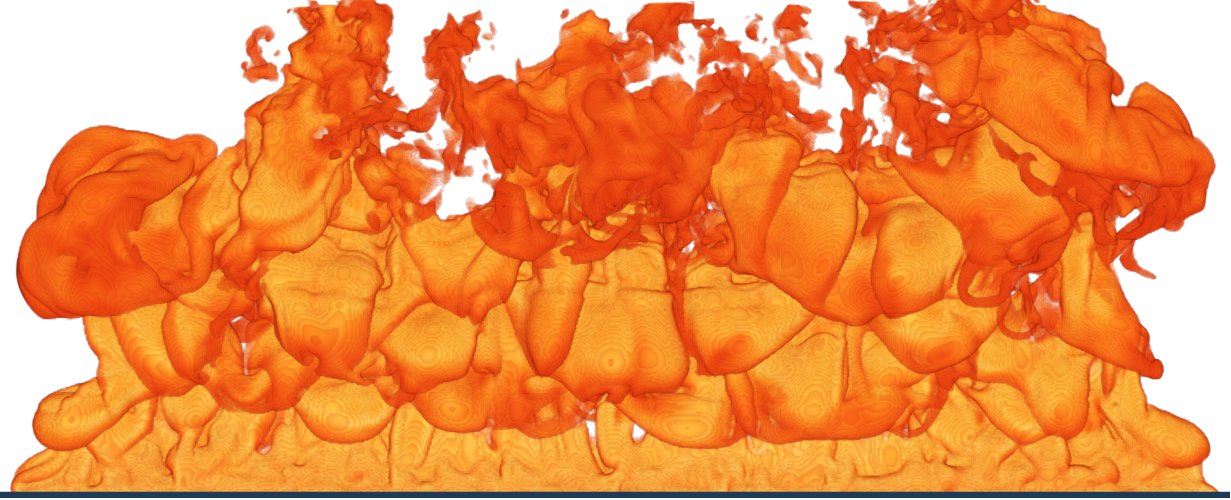
\includegraphics{./content/00_overview/figs/fire_banner.png}

This is the first year that we offer this script. The motivation to
create this script is on the one hand to give the participants of the
lecture a possibility to read the contents. And on the other hand, to
make this content freely available to external or former participants.

However, this script is very short and will remain so. Much of the
content is already available in greater depth, so that reference is made
to the relevant passages - instead of simply copying them.

As the script is under development, we welcome constructive suggestions
and your feedback. This way you can support our whole fire science
community.

\textbf{For the University of Wuppertal students: All organisational
information on the procedure can be found on the
\href{https://cce.uni-wuppertal.de/de/lehre/numerische-brandsimulationen.html}{CCE
website on the fire simulations lecture}.}

\section*{Contents of the Lecture
Notes}\label{contents-of-the-lecture-notes}
\addcontentsline{toc}{section}{Contents of the Lecture Notes}

\markright{Contents of the Lecture Notes}

\begin{itemize}
\tightlist
\item
  It is planned, that this script will not only contain the contents of
  the lecture \emph{Fire Simulations} but also other contents linked to
  this lecture, such as \emph{FDS Data Analysis} and \emph{Using High
  Performance Computers for Fire Simulations}. In the course of the
  lecture, we will announce the contents relevant for you accordingly.
\item
  The script also contains exercises for all topics, with and without
  solution paths, but always with a result or the possibility of
  validating your solution.
\item
  Do not print out the script or save it elsewhere. This way you have
  the latest version, which is continuously improved and supplemented
  with content.
\item
  The script will always remain freely accessible.
\item
  The lecture notes and exercises are designed for \textbf{FDS version
  6.7.5}, and thus may not be valid / reproducible for other versions.
\end{itemize}

\section*{Contributors}\label{contributors}
\addcontentsline{toc}{section}{Contributors}

\markright{Contributors}

Contributors to the development of the script and the exercises are (in
alphabetical order):

\begin{itemize}
\tightlist
\item
  Lukas Arnold
\item
  Kristian Börger
\item
  Tristan Hehnen
\item
  Lilli Klein
\item
  Karen de Lannoye
\item
  Keyvan Najarian
\item
  Tássia Quaresma
\item
  Jan Vogelsang
\item
  My Linh Würzburger
\end{itemize}

\section*{Theses}\label{theses}
\addcontentsline{toc}{section}{Theses}

\markright{Theses}

We offer theses (BA, MA, PhD) on many different topics.

\begin{itemize}
\tightlist
\item
  an overview of topics and previously supervised theses can be found on
  the \href{https://cce.uni-wuppertal.de/en/theses/}{thesis website}
\item
  The \href{https://cce.uni-wuppertal.de/en/research/}{overview of our
  publications} can also help you find
\item
  If you are interested, please contact Lukas Arnold
  \href{https://cce.uni-wuppertal.de/en/team/}{@ University of
  Wuppertal} or
  \href{https://www.fz-juelich.de/ias/ias-7/EN/AboutUs/Staff/Current/Arnold_Lukas/main.html}{@
  Forschungszentrum Jülich}
\end{itemize}

\section*{Acknowledgements}\label{acknowledgements}
\addcontentsline{toc}{section}{Acknowledgements}

\markright{Acknowledgements}

The software tools used in the lecture and the creation of the materials
are mostly freely available, open source and developed by volunteers. In
particular, we would like to thank the following teams for their work

\begin{itemize}
\tightlist
\item
  Team of \href{https://github.com/firemodels/fds}{FDS}
\item
  Team of \href{https://github.com/jupyter/jupyter}{Jupyter}
\item
  Team of \href{https://github.com/jupyterlab}{JupyterLab}
\item
  Team of \href{https://github.com/jupyter/jupyter-book}{Jupter Book}
\end{itemize}

\section*{Contact}\label{contact}
\addcontentsline{toc}{section}{Contact}

\markright{Contact}

How to reach us:

\begin{itemize}
\tightlist
\item
  As a participant of the lecture: best via the associated moodle course
\item
  External interested parties best used our email list.
\item
  Contact details for individuals can be found on the
  \href{https://cce.uni-wuppertal.de/en/team/}{staff website}
\end{itemize}

\section*{License}\label{license}
\addcontentsline{toc}{section}{License}

\markright{License}

These lecture notes and tools are licensed under the
\href{http://creativecommons.org/licenses/by-sa/4.0/}{Creative Commons
Attribution-ShareAlike 4.0 International License}.

\part{Introduction}

\chapter*{Team Fire Dynamics}\label{team-fire-dynamics}
\addcontentsline{toc}{chapter}{Team Fire Dynamics}

\markboth{Team Fire Dynamics}{Team Fire Dynamics}

The \emph{Team Fire Dynamics} is a joint team of members of the chair of
\href{https://cce.uni-wuppertal.de/en.html}{Computational Civil
Engineering (CCE)} at the University of Wuppertal (BUW) and the
\href{https://www.fz-juelich.de/ias/ias-7/EN/Research/Fire_Dynamics/_node.html}{Fire
Dynamics} division, which is part of the
\href{https://www.fz-juelich.de/ias/ias-7}{Institute for Advanced
Simulation (IAS-7)} at the
\href{https://www.fz-juelich.de}{Forschungszentrum Jülich (FZJ)}.

The CCE chair is mainly concerned with the research and development of
new computer-based models. The focus of the application here is fire and
smoke propagation in buildings.

In teaching, we focus on computer science and numerics. The main
lectures we offer are
\href{https://cce.uni-wuppertal.de/index.php?id=4178&L=0}{Computer
Science} and
\href{https://cce.uni-wuppertal.de/index.php?id=4185&L=0}{Fire
Simulations}. In addition to this, we regularly offer workshops on
\emph{data analysis} and \emph{Raspberry Pi}.

The simulation models we develop and use are mostly based on
computational fluid dynamics (CFD). In addition, we use genetic
optimisation algorithms and image processing methods. What they all have
in common is the use of parallel computers, such as the supercomputer
\href{https://www.fz-juelich.de/ias/jsc/EN/Expertise/Supercomputers/JURECA/JURECA_node.html}{JURECA}
at the
\href{https://fz-juelich.de/portal/DE/Home/home_node.html}{Forschungszentrum
Jülich}.

\begin{figure}

\centering{

\includegraphics[width=0.8\textwidth,height=\textheight]{index_files/mediabag/image.jpg}

}

\caption{\label{fig-jureca}JURECA supercomputer. Source:
Forschungszentrum Jülich}

\end{figure}%

Our research activities include the use and further development of
\href{https://pages.nist.gov/fds-smv/}{FDS} (Fire Dynamics Simulator),
which can be used to calculate the spread of smoke and fire in
buildings. On the other hand, the development of new simulation tools.
These include, for example, the simulation software
\href{https://github.com/FireDynamics/ARTSS}{ARTSS} (Accelerator-based
Real-Time Smoke Simulator) or
\href{https://github.com/FireDynamics/propti}{PROPTI}. The research is
carried out in close cooperation with the
\href{https://www.fz-juelich.de/ias/ias-7/EN/Research/Fire_Dynamics/_node.html}{Fire
Dynamics} department at the Jülich Research Centre.

\begin{longtable}[]{@{}
  >{\centering\arraybackslash}p{(\columnwidth - 0\tabcolsep) * \real{1.0000}}@{}}
\toprule\noalign{}
\begin{minipage}[b]{\linewidth}\centering
\end{minipage} \\
\midrule\noalign{}
\endhead
\bottomrule\noalign{}
\endlastfoot
Simulation of fires in an underground station, part of the
\href{http://www.orpheus-projekt.de}{ORPHEUS project}, using the
software \href{https://pages.nist.gov/fds-smv/}{FDS}. \\
\end{longtable}

\begin{longtable}[]{@{}
  >{\centering\arraybackslash}p{(\columnwidth - 0\tabcolsep) * \real{1.0000}}@{}}
\toprule\noalign{}
\begin{minipage}[b]{\linewidth}\centering
\end{minipage} \\
\midrule\noalign{}
\endhead
\bottomrule\noalign{}
\endlastfoot
Simulation of a liquid fire with the software
\href{https://www.openfoam.com/}{OpenFoam} \\
\end{longtable}

\begin{longtable}[]{@{}
  >{\centering\arraybackslash}p{(\columnwidth - 0\tabcolsep) * \real{1.0000}}@{}}
\toprule\noalign{}
\begin{minipage}[b]{\linewidth}\centering
\end{minipage} \\
\midrule\noalign{}
\endhead
\bottomrule\noalign{}
\endlastfoot
Self-consistent simulation of fire spread along a cable route, part of
Hehnen, Arnold, and Mendola (2020). Calculated with
\href{https://pages.nist.gov/fds-smv/}{FDS}. \\
\end{longtable}

\chapter*{References}\label{references}
\addcontentsline{toc}{chapter}{References}

\markboth{References}{References}

\phantomsection\label{refs}
\begin{CSLReferences}{1}{0}
\bibitem[\citeproctext]{ref-Hehnen.2020}
Hehnen, Tristan, Lukas Arnold, and Saverio La Mendola. 2020.
{``{Numerical Fire Spread Simulation Based on Material Pyrolysis---An
Application to the CHRISTIFIRE Phase 1 Horizontal Cable Tray Tests}.''}
\emph{Fire} 3 (3): 33. \url{https://doi.org/10.3390/fire3030033}.

\end{CSLReferences}

\part{Modeling}

\chapter{Modelling Fires}\label{modelling-fires}

The motivation for this chapter is to provide an overview of the
involved phenomena and methods in the modelling of fires. In the first
section a brief summary of the physical and chemical processes is given.
As one of the application scenarios for fire simulations is fire safety
engineering (FSE), the second section outlines some selected aspects of
this field of engineering --~especially for those who are not familiar
with it.

There exist multiple ways to model fires, although this lecutre focuses
on field models, i.e.~computational fluid dynamics models. In the third
section an overview of existing modelling approaches is briefly
outlined.

\section{Physical and Chemical
Processes}\label{physical-and-chemical-processes}

\subsection{What is a Fire?}\label{what-is-a-fire}

In general: A fire is an exothermic chemical reaction.

\textbf{Technical Combustion -- Wanted Fires}

\begin{figure}

\centering{

\includegraphics[width=0.6\textwidth,height=\textheight]{index_files/mediabag/858px-Gas_flame.jpg}

}

\caption{\label{fig-wanted-fire}In a gas stove, a combustible gas is
used to generate heat. The geometry and flow properties of the stove
allow a controllable flame. Source:
\href{https://commons.wikimedia.org/wiki/File:Gas_flame.jpg}{Wikimedia
Commons}.}

\end{figure}%

\emph{Wanted fires}, i.e.~technical combustion processes, are
\textbf{controlled} processes used for e.g.~heating or propulsion.
Although the term \emph{wanted fire} is somehow misleading, as the fires
are typically not wanted and associated with accidents, a bonfire is one
of the fundamental wanted applications of fires.

\begin{figure}

\centering{

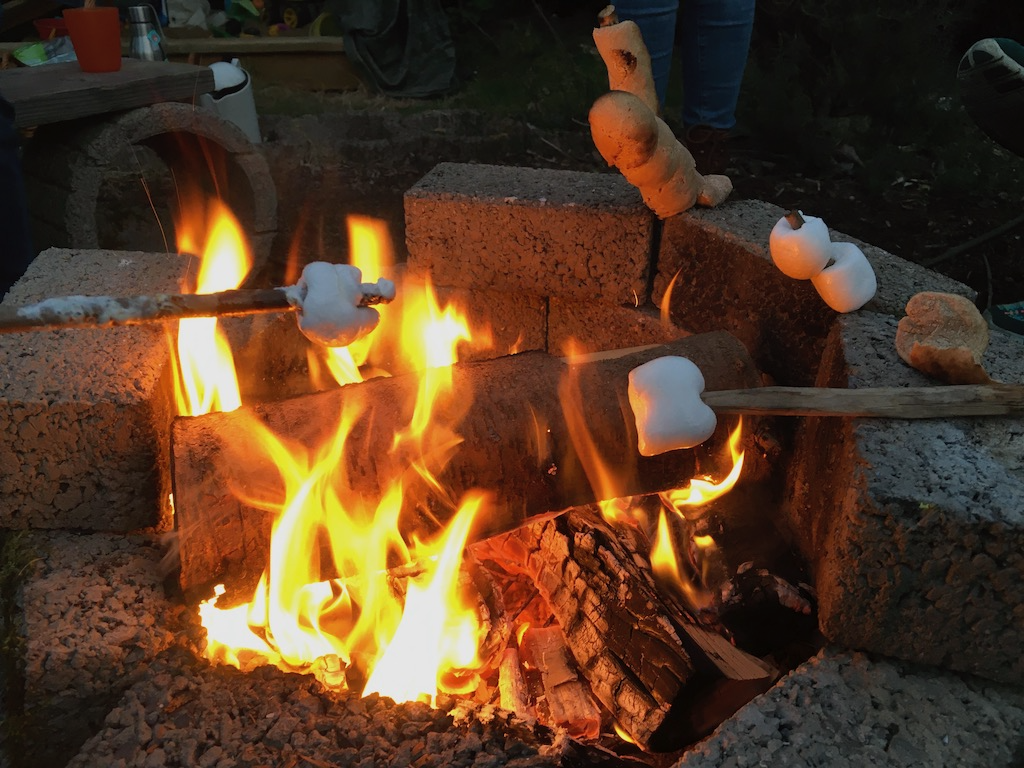
\includegraphics[width=0.4\textwidth,height=\textheight]{content/01_Modeling/01_general/figs/bonfire.png}

}

\caption{\label{fig-bonfire}Bonfires are wanted fires, e.g.~for
preparing a meal.}

\end{figure}%

\textbf{Unwanted Fires}

\begin{figure}

{\centering \includegraphics[width=0.4\textwidth,height=\textheight]{index_files/mediabag/640px-Fire_inside_an.jpg}

}

\caption{Building fire. Source:
\href{https://commons.wikimedia.org/wiki/File:Fire_inside_an_abandoned_convent_in_Massueville,_Quebec,_Canada.jpg}{Wikimedia
Commons}.}

\end{figure}%

Unwanted fires, are \textbf{not controlled and not wanted} processes.
These are mostly incidents inside of enclosures and pose danger to
wildlife, humans, and property.

\textbf{Fire Examples}

\begin{itemize}
\tightlist
\item
  Bonfire

  \begin{itemize}
  \tightlist
  \item
    \href{https://youtu.be/NUKKzdVy0EI}{Lakeside Bonfire}
  \item
    \href{https://uni-wuppertal.sciebo.de/s/e0c3Ut8OolZGTC8}{Slowmotion
    Bonfire}
  \end{itemize}
\item
  Wildland fires

  \begin{itemize}
  \tightlist
  \item
    \href{https://youtu.be/6y0__CZI-Cw}{Walking With Fire: A Wildfire
    Documentary}
  \item
    \href{https://youtu.be/2qYzTU0q9XE}{Indonesia Peat Fires}
  \end{itemize}
\item
  Compartment fires

  \begin{itemize}
  \tightlist
  \item
    \href{https://youtu.be/w4W82HIzUcc}{Compartment Fire Flashover}
  \item
    \href{https://youtu.be/xzuNVFn0U48}{Storage Fire}
  \end{itemize}
\end{itemize}

\subsection{Processes Overview}\label{processes-overview}

\begin{figure}

\centering{

\includegraphics[width=0.8\textwidth,height=\textheight]{index_files/mediabag/content/01_Modeling/01_general/figs/fire_processes.pdf}

}

\caption{\label{fig-fire-processes}Visualisation of the main processes
involved in fires.}

\end{figure}%

Fires involve a complex interaction of a multitude of physical and
chemical processes. While most of them take place in the gas phase,
e.g.~combustion, fires commonly include also processes in the solid or
liquid phase, e.g.~pyrolysis which generates the fuel for the
combustion. The following processes cover the main phenomena.

\begin{enumerate}
\def\labelenumi{\arabic{enumi}.}
\tightlist
\item
  \textbf{Fluid dynamics}

  \begin{itemize}
  \tightlist
  \item
    fundamental mass and momentum transport process in the gas phase
  \item
    fire related flows are mostly turbulent
  \end{itemize}
\item
  \textbf{Heat transfer}

  \begin{itemize}
  \tightlist
  \item
    warm gas, e.g.~combustion products, are transported upwards by heat
    convection
  \item
    hot matter emits net thermal radiation
  \item
    heat conduction inside the solid
  \end{itemize}
\item
  \textbf{Combustion}

  \begin{itemize}
  \tightlist
  \item
    fast oxidation of fuel in the flame
  \item
    release of chemical energy, e.g.~locally heating gas or thermal
    radiation
  \end{itemize}
\item
  \textbf{Pyrolysis}

  \begin{itemize}
  \tightlist
  \item
    degradation of the solid structure
  \item
    emission of volatile gases, e.g.~fuel for the combustion
  \end{itemize}
\end{enumerate}

\subsection{Fluid Dynamics}\label{fluid-dynamics}

Fires induce heat in the gas phase and buoyancy of the heated gas drives
a plume. Compartment flows are complex and involve many openings to
ambient regions as well as obstructions, see
Figure~\ref{fig-compartment-flow}. Mechanical ventilation, systems for
heating, ventilation and air conditioning (HVAC) as well as wind might
be included into the evaluation of the dynamics.

\begin{figure}

\centering{

\includegraphics[width=0.8\textwidth,height=\textheight]{index_files/mediabag/content/01_Modeling/01_general/figs/compartment_flow_labeled.pdf}

}

\caption{\label{fig-compartment-flow}Illustration of a potential flow
inside a building, driven by the heat released by the fire. There is an
inflow and an outflow, which connect the confined flow to the ambient
domain.}

\end{figure}%

Most fire flows, especially in the flame and plume region, are
turbulent. The turbulent mixture process during combustion is crucial
and the entrainment of fresh cold air into a plume significantly
determines its dynamics. Experimental analysis as well as numerical
models must consider the macroscopic effects of turbulence.

\begin{figure}

\centering{

\includegraphics[width=0.4\textwidth,height=\textheight]{index_files/mediabag/466px-Laminar-turbul.jpg}

}

\caption{\label{fig-turbulence-transition-candle}Transition from a
laminar to a turbulent flow in the plume of a burning candle. The image
is captured using
\href{https://en.wikipedia.org/wiki/Schlieren_photography}{schlieren
photography}, which visualises differences in the refraction index.
Source:
\href{https://commons.wikimedia.org/wiki/File:Laminar-turbulent_transition.jpg}{Wikimedia
Commons}.}

\end{figure}%

\subsection{Reactive Flows}\label{reactive-flows}

Fires are driven by the energy released by combustion, which is an
exothermal chemical process. In the simplest case, two gas species, here
oxygen and fuel, react and release energy. In real fires, there is a zoo
of species and reactions involved. Depending on the concentrations of
individual species and their local temperatures, new chemical species
can be formed. Thus, the overall spectrum of products, due to the
chemical processes during a fire, is rarely simple.

In contrast to technical combustion, in fires the oxygen and the fuel
are typically not mixed. The transition from a non-premixed to a
premixed combustion can be well observed with a Bunsen burner, see
Figure~\ref{fig-bunsen-burner}.

\begin{figure}

\centering{

\includegraphics[width=0.4\textwidth,height=\textheight]{index_files/mediabag/854px-Bunsen_burner_.jpg}

}

\caption{\label{fig-bunsen-burner}Variable oxygen concentrations in the
outflow stream of a Bunsen burner. From left to right: air valve closed,
nearly fully closed, valve semi-opened and maximally opened. Source:
\href{https://commons.wikimedia.org/wiki/File:Bunsen_burner_flame_types.jpg}{Wikimedia
Commons}.}

\end{figure}%

The time scales at which the chemical reactions take place span multiple
orders of magnitude, see Figure~\ref{fig-chem-time-scales}. Typical
combustion processes are much faster than common mass transport
processes in fires.

\begin{figure}

\centering{

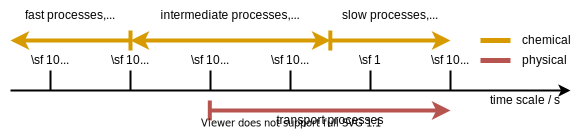
\includegraphics[width=0.8\textwidth,height=\textheight]{index_files/mediabag/content/01_Modeling/01_general/figs/chemical_timescales.pdf}

}

\caption{\label{fig-chem-time-scales}(Very) Approximate time scales of
chemical and physical processes in reactive flows.}

\end{figure}%

\section{Heat Transfer}\label{heat-transfer}

Heat can be transferred between locations and materials in different
ways. The flow of heat is driven by differences in temperature. There
are three modes to transfer heat, where only conduction and radiation
are fundamental and do not require a fluid in a gravity field.

The heat transfer modes are:

\begin{itemize}
\tightlist
\item
  \textbf{Convection:} transport of matter with different temperatures
  due to induced buoyant flows
\item
  \textbf{Conduction:} diffusion of heat in a material
\item
  \textbf{Radiation:} emission and absorption of electro-magnetic waves
\end{itemize}

\begin{figure}

\centering{

\includegraphics[width=0.4\textwidth,height=\textheight]{index_files/mediabag/Heat-transmittance-m.jpg}

}

\caption{\label{fig-heat-transfer-overview}Schematic illustration of the
various heat transfer modes. Source:
\href{https://commons.wikimedia.org/wiki/File:Heat-transmittance-means2.jpg}{Wikimedia
Commons}.}

\end{figure}%

All three modes are important for fires. The released chemical energy
from combustion locally heats up the gas, which changes its density and
is thus affected by buoyancy. Beside the local heating, the hot gas
emits thermal radiation in all directions. Thus, in case of a
compartment fire, it transfers heat towards the walls or other
structures, and e.g.~towards the solid, which provides the fuel source
for the fire. Thus, the solid's surface heats up and heat conduction
spreads the absorbed energy through the solid.

\section{Pyrolysis}\label{pyrolysis}

Pyrolysis describes the emission of (potentially combustible) gases out
of solid material. In general, this is dependent on the solid's
temperature as the decomposition reactions require energy. For liquids,
additional evaporation can take place.

In case of burning wood, like a match in Figure~\ref{fig-burning-match},
the solid material itself is not part of the combustion, but delivers
only the fuel for the fire. Not all material is gasified and a char
residue is left.

\begin{figure}

\centering{

\includegraphics[width=0.4\textwidth,height=\textheight]{index_files/mediabag/Streichholz.jpg}

}

\caption{\label{fig-burning-match}Burning match, where the fuel for the
combustion is emitted by the wood through pyrolysis. Source:
\href{https://commons.wikimedia.org/wiki/File:Streichholz.JPG}{Wikimedia
Commons}.}

\end{figure}%



\end{document}
